% !TeX root=main.tex
\chapter{روش تحقیق}
%\thispagestyle{empty} 
\section{نوع پژوهش}
پژوهش حاضر از نوع توصیفی-همبستگی است.
\section{تعریف متغیر‌ها}
% ^ %%%%%%%%%%%%%%%%%%%%%%%%%%%%%%%%%%%%%%%%%%%%%%%%%%%%%%%%%%%%%
% ^ %%%%%%%%%%%%%%%%%%%%%%%%%%%%%%%%%%%%%%%%%%%%%%%%%%%%%%%%%%%%%
% ^ %%%%%%%%%%%%%%%%%%%%%%%%%%%%%%%%%%%%%%%%%%%%%%%%%%%%%%%%%%%%%

\subsection{تعریف نظری و عملیاتی مشخصات دموگرافیک}


% ^ %%%%%%%%%%%%%%%%%%%%%%%%%%%%%%%%%%%%%%%%%%%%%%%%%%%%%%%%%%%%%
% ^ %%%%%%%%%%%%%%%%%%%%%%%%%%%%%%%%%%%%%%%%%%%%%%%%%%%%%%%%%%%%%
% ^ %%%%%%%%%%%%%%%%%%%%%%%%%%%%%%%%%%%%%%%%%%%%%%%%%%%%%%%%%%%%%
\subsection{تعریف عملیاتی پارامترهای
     نظریه رفتار برنامه ریزی شده    
    % \textit{\gls{Theory of planned behavior}}
}

برای طراحی پرسشنامه جهت سنجش پارامتر‌های تشکیل دهنده ساختار
\textit{\gls{Theory of planned behavior}}
از دستور العمل ارائه شده توسط
\textit{\gls{Icek Ajzen}}
\!\citep{IcekAjzenHomepage}
استفاده شد. این پرسشنامه دارای ۴ سوال، هر یک برای اندازه‌گیری
یکی از پارامترهای نظریه فوق، است.ه

باور
چقدر احتمال دارد که، استفاده شرکت متا و مدیر‌عاملش از این اطلاعات، باعث آسیب‌ دیدن یا متضرر شدن این افراد شود؟ 
خیلی زیاد
زیاد
متوسط
کم
خیلی کم
برای من، آسیبی که افراد بدین وسیله متحمل می‌شوند: 
خیلی اهمیت دارد
نسبتا اهمیت دارد
نمی‌دانم
زیاد اهمیت ندارد
اصلا اهمیت ندارد

هنجار تخصصی
به نظر شما کدام گزینه برای پر کردن جای خالی در جمله زیر، درست‌تر است؟
متخصصین علوم داده(Data Scientist)، فکر می کنند که من ـــــــــ به اینستاگرام اجازه دهم که به اسامی و شماره تلفن‌ افراد، که در گوشی دارم، دسترسی داشته باشد. 
قطعا باید
باید
فرقی نمی‌کند
نباید
قطعا نباید
وقتی مساله به اشتراک گذاشتن اطلاعات خصوصی دیگران مطرح باشد، من می‌خواهم به حرف متخصصین علوم داده عمل کنم. 
کاملا درست است
نسبتا درست است
نه درست است و نه نادرست
درست نیست
اصلا درست نیست

هنجار تخصصی
بیشتر دوستان من اجازه دسترسی برنامه اینستاگرام به لیست اسامی و شماره تلفن‌‌های افراد که در در گوشی‌شان دارند را، نمی‌دهند . 
کاملا درست است
نسبتا درست است
نه درست است و نه نادرست
درست نیست
اصلا درست نیست
وقتی مساله به اشتراک گذاشتن اطلاعات خصوصی دیگران مطرح باشد، چقدر می‌خواهید که
مثل دوستانتان رفتار کنید؟ 
خیلی زیاد
زیاد
متوسط
کم
خیلی کم

کنترل ادراک شده
« من توانمندی دارم که به برنامه اینستاگرام اجازه دسترسی به لیست اسامی و شماره تلفن های ذخیره در گوشی‌ام را، ندهم.» 
کاملا درست است
نسبتا درست است
نه درست است و نه نادرست
درست نیست
اصلا درست نیست

نیت
«من قصد دارم، به برنامه اینستاگرام اجازه بدهم تا به لیست اسامی و شماره تلفن های ذخیره در گوشی‌ام، دسترسی داشته باشد.» 
کاملا درست است
نسبتا درست است
نه درست است و نه نادرست
درست نیست
اصلا درست نیست

تصمیم
«برنامه اینستاگرام ، همین الان، به لیست اسامی و شماره تلفن های ذخیره در گوشی‌ام، دسترسی دارد.» 
بله
خیر

برای طراحی این پرسشنامه از تحقیقی که در سال ۲۰۲۰ انجام شده است الهام گرفته شده است
\!\citep{vanderschyffInformationPrivacyBehavior2020a}.
این تحقیق جهت بررسی رفتار کاربران
\textit{\gls{Facebook}}
در نصب  کردن
\gls{App}
\!‌های
این شبکه اجتماعی انجام شده‌است. این
\gls{App}
\!‌ها
که هر یک سرویس‌های مورد علاقه کاربران را ارائه می‌کنند، می‌توانند به همه یا بخشی از اطلاعات شخصی
کاربر و دوستان او در
\gls{Facebook}
دسترسی پیدا کنند. نمونه یکی از همین
\gls{App}
\!‌ها
در سال ۲۰۱۳ توسط حدود سیصد هزار نفر از کاربران
\gls{Facebook}
نصب شد و با دسترسی پیدا کردن به پروفایل شخصی آنها و دوستان آنها،
اطلاعات هشتاد و هفت میلیون‌ نفر را استخراج کند
\citep{confessoreCambridgeAnalyticaFacebook2018,salinasZuckerbergCambridgeAnalytica,smithThereOpenSecret}.
سوء استفاده و به اشتراک گذاری مجدد این اطلاعات بعدا باعث
به وجود آمدن
\gls{Cambridge Analytica scandal}
در سال ۲۰۱۶ شد
\!\citep{gonzalezGlobalReactionsCambridge2019,SuspendingCambridgeAnalytica2018}.
سوالات طراحی شده در جدول
\eqref{tab:TPBquestions}
درج شده‌اند.

\begin{table}[ht]
    \caption{سوال‌ها و پارامتر‌های \gls{Theory of planned behavior}}
    \label{tab:TPBquestions}
    \centering
    \onehalfspacing
    % \begin{tabular}{p{0.35\linewidth} | p{0.6\linewidth}}  
    \begin{tabularx}{\linewidth}{ r X }
        % \hline 
        پارامتر
         &
        % درجه آزادی 
        % تبدیل مختصات &
        سوال
        \\
        \hline
        \gls{Atteutude}
         &
        % zotero://select/library/items/LCYS3GQ2
        % https://www.zotero.org/users/5038267/items/LCYS3GQ2
        %توضیحو
        آخرین باری که برنامه
        \gls{Whasapp}
        نصب کردم، از من درخواست کرد که
        به لیست همه اسامی و شماره تلفن‌های‌ ذخیره
        در گوشی‌ من، دسترسی داشته باشد
        \!.نظر شما چیست؟

        ۱-خیلی خوب است
        ۲-خوب است
        ۳-نه خوب است نه بد
        ۴-بد است
        ۵-خیلی بد است
        \\
        \gls{Subjective norm}
         &

        به نظر من، همه دوستانم اگر امروز برنامه
        \gls{Whasapp}
        را دوباره نصب کنند، اجازه می دهند که
        به لیست همه اسامی و شماره تلفن‌های‌ ذخیره
        در گوشی‌شان، دسترسی داشته باشد.

        چقدر از این موضوع اطمینان دارید؟

        ۱-کاملا مطمئنم
        ۲-نسبتا مطمئنم
        ۳-نظری ندارم
        ۴-زیاد مطمئنم نیستم
        ۵-اصلا مطمئنم نیستم
        % مثال‌ها;
        % \lr{S1}:
        % \lr{S1}:
        % \lr{S1}:
        \\
        \gls{Perceived Behavioral control}
         &
        اگر من امروز برنامه
        \gls{Whasapp}
        را دوباره نصب کنم، اجازه دسترسی به
        لیست اسامی و شماره تلفن های
        ذخیره در گوشی‌ام را، خواهم داد.

        آیا می‌توانید اجازه ندهید؟

        ۱-کاملا می‌توانم
        ۲-شاید بتوانم
        ۳-نمی‌دانم
        ۴-شاید نتوانم
        ۵-اصلا نمی‌توانم

        % \hline 
        \\
        \gls{Intention}
         &
        من قصد دارم که اگر امروز برنامه
        \gls{Whasapp}
        را دوباره نصب کنم و اجازه دسترسی
        به لیست اسامی و شماره تلفن های
        ذخیره در گوشی‌ام را بدهم.

        چقدر از این موضوع اطمینان دارید؟

        ۱-حتما می‌دهم
        ۲-شاید بدهم
        ۳-نمی‌دانم
        ۴-شاید ندهم
        ۵-اصلا نمی‌دهم
        % \hline 
        \\
    \end{tabularx}
\end{table}
% ^ %%%%%%%%%%%%%%%%%%%%%%%%%%%%%%%%%%%%%%%%%%%%%%%%%%%%%%%%%%%%%
% ^ %%%%%%%%%%%%%%%%%%%%%%%%%%%%%%%%%%%%%%%%%%%%%%%%%%%%%%%%%%%%%
% ^ %%%%%%%%%%%%%%%%%%%%%%%%%%%%%%%%%%%%%%%%%%%%%%%%%%%%%%%%%%%%%

\subsection{تعریف نظری متغیر جهت‌گیری ارزش اجتماعی}
\textit{
    \textbf{
        \gls{Social Value Orientations}
    }
}
عناوین مختلفی برای اشاره به انگیزه‌هایی که شالوده
\gls{Interdependent decision behavior}
را تشکیل می‌دهند، به کار برده شده است
\!:
\!,
\textit{
    \gls{Welfare tradeoff ratios}
}
\!,
\textit{
    \gls{Other-regarding preferences}
}
\!,
\textit{
    \gls{Social motives}
}
\!,
\!,
\textit{
    \gls{Social preferences}
}
و در پایان
\textit{
    \gls{Social Value Orientations}
}
\!\citep{murphyMeasuringSocialValue2011}.
تاثیر گرفتن نسبی این انگیزه‌ها از دریافتی فرد دیگر که
در پژوهش‌های مختلف نشان داده شده است، پیش‌فرض‌های
\textit{
    \gls{Rational choice theory}
}
را به چالش می‌کشند.از این پیش‌فرض‌ها با عنوان
\textit{
    \gls{Selfishness axiom}
}
نام برده شده است
\!\citep{henrichEconomicManCrosscultural2005}.

در غالب چارچوب
\gls{Social Value Orientations}
فرض می‌شود که افراد از نظر هدف یا انگیزه با یکدیگر تقاوت دارند. این
تفاوت در ارزیابی آنها در تقسیم یک دارایی میان خود
و فرد دیگر ظاهر می‌شود. به عنوان مثال ممکن است فرد تصمیم گیرنده
تلاش کند تا دریافتی خودش را حداکثر کند
\textit{
    \!(\gls{Individualistic})
}،
یا تلاش کند که دریافتی مشترک‌اش را با فرد دیگر حداکثر کند
\!(\gls{Prosocial}).
به همین ترتیب ممکن است تلاش کند تفاوت دریافتی خود و فرد دیگر را حداکثر کند
\textit{
    \!(\gls{Competitive})
}
و
یا آن‌را حداقل کند
\textit{
    \!(\gls{Inequality averse})
}.
به این ترتیب
\textit{
    \gls{Selfishness axiom}
}
به صورت یک نوع خاص از
\textit{
    \gls{Social Value Orientations}
}
در می‌آید که کاملا
\textit{
    \gls{Individualistic}
}
است. گفتنی است که فرض کردن طیف‌های متفاوتی از
\textit{
    \gls{Social Value Orientations}
}
فرض
\textit{
    \gls{Rational choice theory}
}
را به چالش نمی‌کشد بلکه به عنوان افزونه‌ای برای افزایش
\textit{
    \gls{Psychological realism}
}
و
\textit{
    \gls{Descriptive accuracy}
}
این نظریه به کار می‌رود.

نشان داده شده است که
\textit{
    \gls{Social Value Orientations}
}
بر روی
\textit{
    \gls{Cognition}
}
تاثیر می‌گذارد و سبب‌ساز ایجاد رفتار در زمینه‌های متفاوت
\textit{
    \gls{Interpersonal decision making}
}،
به ویژه در
\textit{
    \gls{Negotiation settings}
}
\!\citep{dedreuShareShareAlike1998}
و
\textit{
    \gls{Resource dilemma}
}
\!\citep{rochCognitiveLoadEquality2000,rochEffectsEnvironmentalUncertainty1997,samuelsonMultiattributeEvaluationApproach1993}
می‌گردد.
\textit{
    \gls{Social Value Orientations}
}
همچنین به عنوان
\textit{
    \gls{Covariate}
}
در تعامل با حالات  هیجانی مختلف، تمایل به همکاری را تحت تاثیر قرار می‌دهد
\citep{zeelenbergEmotionSpecificityDecision2008}.
\gls{Social Value Orientations}
در
\textit{
    \gls{Non-human primate}
}
نیز مشاهده شده است که  نشان می‌دهد، بعضی از دیگر گونه‌ها نیز رفتار
\gls{Prosocial}
از خود نشان می‌دهند.
% ^ %%%%%%%%%%%%%%%%%%%%%%%%%%%%%%%%%%%%%%%%%%%%%%%%%%%%%%%%%%%%%
% ^ %%%%%%%%%%%%%%%%%%%%%%%%%%%%%%%%%%%%%%%%%%%%%%%%%%%%%%%%%%%%%
% ^ %%%%%%%%%%%%%%%%%%%%%%%%%%%%%%%%%%%%%%%%%%%%%%%%%%%%%%%%%%%%%

\subsection{تعریف عملیاتی متغیر جهت‌گیری ارزش اجتماعی}
با توجه به محدودیت‌های ابزار‌هایی که با استفاده از
\textit{
    \gls{Categorical approach}
}
\gls{Social Value Orientations}
را می‌سنجند
(مانند عدم دقت نسبت به تقاوت های فردی آزمودنی‌ها به علت
وضوح پایین، محدود بودن به ایجاد تمایز تنها با استفاده از  تولید
\textit{
    \gls{Nominal categorization}
}
و
عدم تولید نتایج نامتناقض، نیاز به زمان و زحمت زیاد از طرف آزمودنی، عدم
حساسیت کافی برای تشخیص انگیزش‌های ظریف‌تر مانند
\gls{Inequality aversion}
)
\citep{murphyMeasuringSocialValue2011}
از
\textit{
    \gls{SVO Slider Measure}
}
استفاده کردیم. این ابزار
به تفاوت‌های درون فردی و میان فردی حساس است و مقایسه را تسهیل می‌کند
\!.
\textit{
    \gls{SVO Slider Measure}
}
قابلیت استفاده آسانی دارد، کارامد است، می تواند تفاوت‌های بیشتر متداول
فردی را تشخیص دهد،  اجازه ارزیابی رده‌بندی
\textit{
    \gls{Social preferences}
}
را می‌دهد و نتایج با معنی  بار تقریبا همه آزمودنی‌ها ایجاد می‌کند. این
ابزار به نیاز به سنجه‌های با وضوح بالا است، که داده‌های
\textit{
    \gls{Continuous}
}
تولید می‌کند.
این ابزار به صورت یک
\textit{
    \gls{Web interface}
}
طراحی شده است
\!(شکل
\ref{fig:SVOPage01}
)\!.
\begin{figure}[htpb]
    \centering
    
\includegraphics[width=0.8\textwidth]{./img/SVOPage01.png}
    \caption{صفحه نخست}
    \label{fig:SVOPage01}
\end{figure}
\begin{figure}[htpb]
    \centering
    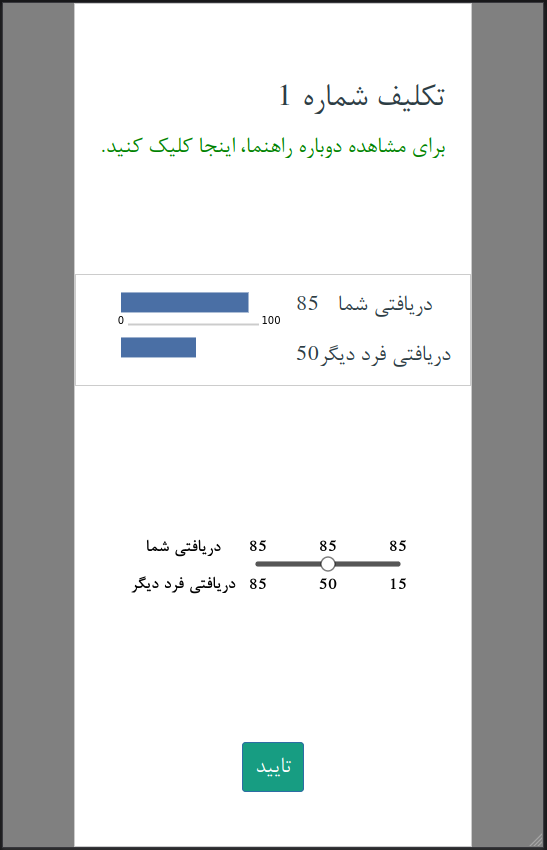
\includegraphics[width=0.8\textwidth]{./img/SVOPage02.png}
    \caption{صفحه تست}
    \label{fig:SVOPage02}
\end{figure}
\begin{figure}[htpb]
    \centering
    
\includegraphics[width=0.8\textwidth]{./img/SVOPage02Instruction.png}
    \caption{راهنمای در دسترس}
    \label{fig:SVOPage02Instruction}
\end{figure}
\begin{figure}[htpb]
    \centering
    
\includegraphics[width=0.8\textwidth]{./img/SVOPageFinal.png}
    \caption{صفحه پایانی}
    \label{fig:SVOPageFinal}
\end{figure}

\textit{
    \gls{Source code}
}
این ابزار به وسیله بسته  نرم‌افزاری
\textit{
    \gls{Next.js}
}
نوشته شده است. به منظور فارسی کردن زبان رابط کاربری و
بهینه کردن بخش‌های مختلف آن برای استفاده در این پژوهش  تغییراتی، در
\gls{Source code}
انجام شد.
در نهایت برای ایجاد یک تجربه پیوسته و بدون وقفه برای آزمودنی‌ها، این ابزار
در بقیه قسمتهای طراحی شده آزمایش، ادغام شد
\!.
این ابزار دارای شش بخش  اصلی و نه بخش ثانویه اختیاری است.  همه بخش‌ها شکل کلی
یکسانی دارند. هر بخش شامل یک وظیفه تصمیم گیری برای تقسیم منابع اشتراکی است. منابع
اشتراکی دارای مقادیر پیوسته هستند که به وسیله حرکت دادن
\textit{
    \gls{Slider}
}
توسط آزمودنی که فرد تصمیم گیرنده است، تغییر می‌کنند. برای مثال فرد تصمیم گیرنده
می‌تواند مقدار
$ x $
را بین ۵۰ و ۱۰۰ که شامل هر دو عدد نیز می‌شود، را انتخاب کند. دریافتی او مقدار
$ x $
خواهد بود در حالی‌که به فرد دیگر
$ 150 - x $
می‌رسد. شمارنده‌های موجود در صفحه مقادیری که در هر لحظه به دو طرف میرسد را، همراه با
جابجا شدن
\textit{
    \gls{Slider}
}
بر روی
\textit{
    \gls{Slider bar}
}
نشان می‌دهند. همزمان  دو نمودار میله‌ای افقی به صورت بصری کم و زیاد شدن
سهم طرفین را به صورت کیفی، با تغییر  اندازه نمایش می‌دهند. وقتی که
آزمودنی
\textit{
    \gls{Slider}
}
را بر روی مقدار مورد پسند خود قرار داد، می‌تواند دکمه تایید را فشار دهد تا اطلاعات این بخش ذخیره شوند
\!\citep{darchePdarcheSvoApplication}.

% & %%%%%%%%%%%%%%%%%%%%%%%%%%%%%%%%%%%%%%%%%%%%%%%%%%%%%%%%%%%%%
% & %%%%%%%%%%%%%%%%%%%%%%%%%%%%%%%%%%%%%%%%%%%%%%%%%%%%%%%%%%%%%
% ^ %%%%%%%%%%%%%%%%%%%%%%%بقیه اش نوشته شود%%%%%%%%%%%%%%%%%%%%%%%%%%%%%%%%%%%%%%
% eck for transitivity in her revealed preferences. The SVO Slider Measure has several advantages. First, the responses can be evaluated for comprehension (e.g., checking the correspondence between the mark on the distribution line and the written distribution values). Second, the responses can be evaluated for transitivity. Although SVO is a matter of subjective preferences, these preferences should conform to the elemental requirement of transitivity. Random responding would likely result in an intransitive set of responses. Third, the responses yield a full ranking of preferences over motivations. Fourth, the measure can be scored in a straight-forward manner to yield a single index of SVO as follows. The mean allocation for self ( ̄ A s) is computed as is the mean allocation for the other ( ̄ A o). Then 50 is subtracted from each of these means in order to “shift” the base of the resulting angle to the center of the circle (50, 50) rather than having its base start at the Cartesian origin. Finally, the inverse tangent of the ratio between these means is computed, resulting in a single index of a person’s SVO.
این ابزار یک عدد که نمایان‌گر تیپ آزمودنی است را به عنوان خروجی بر اساس میانگین مقادیر واگذار شده به خود و دیگری، 
به عنوان خروجی ارائه می‌کند.
% ^ %%%%%%%%%%%%%%%%%%%%%%%%%%%%%%%%%%%%%%%%%%%%%%%%%%%%%%%%%%%%%
% ^ %%%%%%%%%%%%%%%%%%%%%%%%%%%%%%%%%%%%%%%%%%%%%%%%%%%%%%%%%%%%%
% ^ %%%%%%%%%%%%%%%%%%%%%%%%%%%%%%%%%%%%%%%%%%%%%%%%%%%%%%%%%%%%%
\subsection*{تعریف نظری متغیر تصمیم گیری به اشتراک گذاری اطلاعات خصوصی دیگران}
افراد در موقعیت‌های زیادی با شرایط تصمیم گیری برای انتخاب میان
به اشتراک گذاری اطلاعات شخصی خود و نگه داشتن آن نزد خود، روبرو می‌شوند.
آنها در این شرایط سود و یا زیان خود را در نظر می‌گیرند
\!\citep{dinevExtendedPrivacyCalculus2006b,dienlinExtendedPrivacyCalculus2016}
\!.
تصمیم‌ گیری برای به  اشتراک گذاشتن اطلاعات شخصی دیگران، ملاحظات اجتماعی را به همراه دارد.
در این شرایط فرد تصمیم گیرنده، منفعتی که با به اشتراک گذاری اطلاعات شخصی دیگران به دست می آورد را
با کنترلی که فرد دیگر بر روی اطلاعات شخصی خود دارد و یا با
\textit{
    \gls{Information privacy}
}
سبک و سنگین می‌کند
\!
\!\citep{kamleitnerYourDataMy2019,puModelFactorsInfluencing2016}
\!.
\subsection*{تعریف عملیاتی متغیر تصمیم گیری به اشتراک گذاری اطلاعات خصوصی دیگران}
در این پژوهش از شبیه‌سازی یک موقعیت واقعی برای آزمودنی برای اندازه‌گیری رفتار او استفاده کردیم. در این شبیه‌سازی 
از آزمودنی درخواست شد که فرد یا افراد دیگری را حداکثر تا پنج نفر به عنوان آزمودنی جدید برای شرکت 
در آزمایش معرفی کند. جمع‌آوری نمونه به شیوه گلوله برفی در پژوهش‌های انسانی  به همین صورت  انجام می‌شود با این 
تفاوت که در آزمایش ما، افراد معرفی شده برای انجام آزمایش دعوت نشدند. تنها از شاخص‌های آماری تعداد افراد 
معرفی شده در بخش‌های مختلف آزمایش برای صحت‌سنجی فرضیه‌های آزمایشی این پژوهش استفاده شد. فاش‌سازی
 شماره تلفن و نام و نام خانوادگی که آزمودنی از دوستان و آشنایان خود در اختیار دارد برای شرکت در آزمایش، به
 عنوان شاخص تصمیم‌گیری برای به اشتراک گذاری اطلاعات خصوصی دیگران اندازه‌گیری شده است.
% ^ %%%%%%%%%%%%%%%%%%%%%%%%%%%%%%%%%%%%%%%%%%%%%%%%%%%%%%%%%%%%%
% ^ %%%%%%%%%%%%%%%%%%%%%%%%%%%%%%%%%%%%%%%%%%%%%%%%%%%%%%%%%%%%%
% ^ %%%%%%%%%%%%%%%%%%%%%%%%%%%%%%%%%%%%%%%%%%%%%%%%%%%%%%%%%%%%%
% ^ %%%%%%%%%%%%%%%%%%%%%%%%%%%%%%%%%%%%%%%%%%%%%%%%%%%%%%%%%%%%%
% ^ %%%%%%%%%%%%%%%%%%%%%%%%%%%%%%%%%%%%%%%%%%%%%%%%%%%%%%%%%%%%%
% ^ %%%%%%%%%%%%%%%%%%%%%%%%%%%%%%%%%%%%%%%%%%%%%%%%%%%%%%%%%%%%%
\subsection{تعریف نظری متغیر
    \textit{هنجار ذهنی }
    و
    \textit{باور هنجاری از ارزش اطلاعات}
    خصوصی دیگران}
    \textit{
        \gls{Subjective norm}
    }
    و
    \textit{
        \gls{Normative belief}
    }
    دو مفهوم اساسی هستند که نگرش فرد نسبت به هنجار اجتماعی نسبت به یک موضوع را در 
    نظریه رفتار برنامه‌ریزی شده
    تعریف می‌کنند. 
    باور هنجاری
    ، ادراک فرد از فشار‌های هنجارهای اجتماعی،  و یا باورهای دیگران 
    به اینکه چه رفتاری باید یا نباید انجام شود. 
    هنجار ذهنی
    ادراک فرد درباره یک رفتار مشخص است که تحت تاثیر قضاوت افراد مهم زندگی 
فرد، قرار دارد. 
در اینجا رفتاری که مد نظر قرار دارد تصمیم‌گیری برای مشخص کردن مبلغ پولی که برای خرید  یک مجموعه داده مشخصی از اطلاعات 
شخصی دیگران لازم است، می‌باشد.
    \!\citep{amjadIdentifyingChangingNormative2009}
% ^ %%%%%%%%%%%%%%%%%%%%%%%%%%%%%%%%%%%%%%%%%%%%%%%%%%%%%%%%%%\!\citep{kamleitnerYourDataMy2019,amjadIdentifyingChangingNormative2009}%%%
% ^ %%%%%%%%%%%%%%%%%%%%%%%%%%%%%%%%%%%%%%%%%%%%%%%%%%%%%%%%%%%%%
% ^ %%%%%%%%%%%%%%%%%%%%%%%%%%%%%%%%%%%%%%%%%%%%%%%%%%%%%%%%%%%%%
% ^ %%%%%%%%%%%%%%%%%%%%%%%%%%%%%%%%%%%%%%%%%%%%%%%%%%%%%%%%%%%%%
% ^ %%%%%%%%%%%%%%%%%%%%%%%%%%%%%%%%%%%%%%%%%%%%%%%%%%%%%%%%%%%%%
% ^ %%%%%%%%%%%%%%%%%%%%%%%%%%%%%%%%%%%%%%%%%%%%%%%%%%%%%%%%%%%%%
% \subsection{تعریف عملیاتی متغیر
%     \textit{هنجار ذهنی }
%     و
%     \textit{باور هنجاری از ارزش اطلاعات}
%     خصوصی دیگران}
% برای اندازه‌گیری
% \textit{
%     \gls{Subjective norm about information value}
% }
% و
% \textit{
%     \gls{Normative belief about information value}
% }
% از پرسشنامه پژوهش‌گر ساخته
% \textit{
%     \gls{Dataset valuation invetory}
% }
% استفاده شد.
% این ابزار دارای ۱۴ سوال است که دسته‌های هفت‌گانه داده‌های شخصی دیگران را مورد ارزش‌یابی قرار می‌دهد.
% پژوهشی که برای یافتن ابعاد اطلاعات شخصی بر اساس نوع خطری که افراد
% از فاش شدن آن احساس لحاظ می‌کنند، ۷ دسته از اطلاعات شخصی را مشخص کرده‌است
% \citep{karwatzkiMultidimensionalNaturePrivacy}.
% هر یک از این دسته‌ها دارای ۲ سوال در پرسشنامه هستند. در مجموع ۱۴ سوال در این پرسشنامه به آزمودنی ارائه شد.
% %  برای سنجش 
% % پایایی درونی
% % این پرسشنامه سوالات به دو پرسشنامه ۷ سوالی تقسیم شدند.
% % هر یک از این پرسشنامه‌ها دارای یک سوال از هر یک از دسته‌های دسته‌بندی هفت‌گانه اطلاعات، می‌باشند.
% به نیمی از افراد شرکت کننده در آزمایش، به طور تصادفی، پرسشنامه ۷ سوالی شماره یک به همراه سوالی برای سنجیدن
% میزان دقت انجام پرسشنامه توسط آزمودنی 
% به ارزش  مجموعه‌داد مشخصی از اطلاعات  شخصی دیگران، ارائه شد.
% پرسشنامه ۷ سوالی شماره ۲ نیز به همراه سوالی برای سنجش باور فرد نسبت به ارزشی که دیگران 
% برای یک مجموعه‌داده مشخصی قائل هستند، پس از پرسشنامه اول داده شد.

% به نیمی دیگر از افراد که آنها نیز به طور تصادفی انتخاب شدند، همین دو پرسشنامه، اما با ترتیب بر عکس از دو سوال نامبرده شده  ارائه شدند.
% برای اطمینان از پایایی درونی پرسشنامه و بررسی امکان وجود 
% اثر ترتیب
% سوالات با دو ترتیب که کاملا برعکس هم هستند ارائه شدند.
% آزمودنی با استفاده از  یک
% دکمه کشویی
% مقدار ارزشی که تعیین کرده است را از بین ۰ تا ۱۰۰ انتخاب می‌کند.
% امتیازاتی که آزمودنی ها به سوال شماره یک داده‌اند، به عنوای معیاری برای سنجش 
% نگرش به ارزش اطلاعات خصوصی دیگران
% به کار گرفته شده است.
% امتیازات به سوال شماره دو نیز به همین صورت برای 
% سنجش
% باور هنجاری نسبت به ارزش اطلاعات خصوصی دیگران
% به کار رفت. 77



% ^ %%%%%%%%%%%%%%%%%%%%%%%%%%%%%%%%%%%%%%%%%%%%%%%%%%%%%%%%%%%%%
% ^ %%%%%%%%%%%%%%%%%%%%%%%%%%%%%%%%%%%%%%%%%%%%%%%%%%%%%%%%%%%%%
% ^ %%%%%%%%%%%%%%%%%%%%%%%%%%%%%%%%%%%%%%%%%%%%%%%%%%%%%%%%%%%%%
\subsection{تعریف نظری متغیر سه‌گانه تاریک}
\textit{
    \textbf{
        سه‌گانه تاریک
    }
}
\LTRfootnote{
    Dark Triad
}
سه ویژگی شخصیتی
\textit{
    ماکیاولیسم
}
\!،
\LTRfootnote{
    Machiavellianism
}
\textit{
    خودشیفتگی
}
\LTRfootnote{
    Narcissism
}
و
\textit{
    ضداجتماعی
}
\LTRfootnote{
    Psychopathy
}
را در بر می‌گیرد. این سه جنبه می‌توانند شامل افرادی باشند که دارای عملکرد طبیعی هستند و در جامعه حضور دارند
\!\citep{paulhusDarkTriadPersonality2002}
\!.
رفتارهای افراد ماکیاولیسیت به وسیله توانایی او برای توجیه کردن
کارهایشان قابل تشخیص است. از دید آنها هدف وسیله را توجیه
می‌کند. رفتار ضد اجتماعی و ماکیاولیستی دو سازه جدا هستند، هرچند همپوشانی
مفهومی دارند. هر دو سازه، فقر روابط هیجانی-عاطفی و عدم وجود
ملاحظات اخلاقی را در بر می‌گیرند. در رفتار ضد اجتماعی فقدان عاطفه
بیشتر مشاهده می شود
\!\citep{paulhusDarkTriadPersonality2002,vernonBehavioralGeneticInvestigation2008}
اما در رفتار ماکیاولیستی بهره کشی و سوء استفاده وجود دارد.
رفتار ضد اجتماعی تحت تاثیر فقدان گناه، عدم صداقت، بدبینی و
سنگدل بودن قرار دارد.
رفتار یک فرد خودشیفته  در جهت جلب توجه و به دست آوردن موقعیت
اجتماعی است. آنها بر این باور هستند که از دیگران برتری و استحقاق بیشتری دارند
% \citep{furnhamPersonalityTraitsTypes2005}
\!. اختلال شخصیت خودشیفته و اختلال شخصیت ضد اجتماعی در
\textit{
    دی. اس. ام.
}
\!\!\LTRfootnote{
    Diagnostic and Statistical Manual of Mental Disorders(DSM)
}
تعریف شده اند اما رفتار ماکیاولیستی به
عنوان یک اختلال تعریف نشده است. پژوهش‌های پیشین نشان داده است که سه
مؤلفه سه گانه تاریک دارای ابعاد ژنتیکی و درونزاد هستند
\!\citep{kvTraitEmotionalIntelligence2011}
\!.
تنها بعد ماکیاولیستی دارای بعد محیطی بیشتری است و تحت تاثیر تجربه تقویت یا تعدیل می‌شود
\!.
% ^%%%%%%%%%%%%%%%%%%%%%%%%%%%%%%%%%%%%%%%%%%%%%%%%%%%%%%%%%%%%%%%%%%%%%%%%%%%%%%%%%%%%%
% ^%%%%%%%%%%%%%%%%%%%%%%%%%%%%%%%%%%%%%%%%%%%%%%%%%%%%%%%%%%%%%%%%%%%%%%%%%%%%%%%%%%%%%
% ^%%%%%%%%%%%%%%%%%%%%%%%%%%%%%%%%%%%%%%%%%%%%%%%%%%%%%%%%%%%%%%%%%%%%%%%%%%%%%%%%%%%%%
% \subsection{تعریف عملیاتی متغیر‌ها}
\textbf{تعریف عملیاتی سه گانه تاریک}
:
برای سنجش ویژگی‌های ضداجتماعی، ماکیاولیسم و خودشیفتگی از پرسشنامه ۱۲ سوالی ویژگی‌های تاریک، ساخته شده توسط
\textit{
    پیتر جانسون }
\LTRfootnote{
    Peter K. Jonason
}
و
\textit{
    گرگوری وبستر}
\LTRfootnote{
    Gregory D. Webster
}
استفاده کردیم.
\!\citep{jonasonDirtyDozenConcise2010}
\textit{
    روایی سازه
}
\LTRfootnote{
    Construct validity
}
بر اساس دو روایی
\textit{
    روایی همگرا
}
\LTRfootnote{
    Content validity
}
و
\textit{
    روایی افتراقی
}
\LTRfootnote{
    Discriminant validity
}
این پرسشنامه مختصر بر اساس مقایسه پرسشنامه ۹۱ سوالی پیشین مورد تایید قرار گرفته است
\!\citep{jonasonDirtyDozenConcise2010}
\!.
روایی این پرسشنامه برای جامعه ایران توسط
\textit{
    یوسفی
}
و
\textit{
    پیری
}
% ^ %%%%%%%%%%%%%%%%%%%%%%%%%%%%%%Farsi citation
\!\citep{ywsfyWyjgyHyRwn2016}
مورد تایید قرار گرفته است.
برای طراحی نسخه تحت وب این پرسشنامه از پکیج نرم‌افزاری
\textit{
    ری‌اکت
}
\LTRfootnote{
    React
}
و کتابخانه تولید پرسشنامه جاوااسکریپت
\textit{
    سروی جی. اس.
}
\LTRfootnote{
    Surveyjs
}
استفاده شد و برای اندازه گیری رفتار آزمودنی‌ها در زمان انجام آزمایش از کدنویسی جاوااسکریپت استفاده شد
\!.
%  WEB LINK TO THIS PART FOR ZOTERO ANNOTATIONS 001
برای بررسی و رفع اثر عامل
\textit{
    اثر تقدم
}
\LTRfootnote{
    Primacy effects
}
و
\textit{
    اثر ترتیب
}
\LTRfootnote{
    Order effects
}
\!\citep{dillmanMultipleAnswerQuestions2003,krosnickEVALUATIONCOGNITIVETHEORY1987,leeEffectQuestionOrder2009}
و همچنین پرهیز از افزایش واریانس خطا که
با تصادفی سازی کامل همه گزینه‌ها بین آزمودنی‌ها پیش می‌آید،
\!\citep{dillmanMultipleAnswerQuestions2003}
آزمودنی‌ها به طور تصادفی و در زمان آغاز پرسشنامه
توسط الگوریتم به کار رفته در رابط تحت وب، به دو دسته تقسیم
شدند. به دسته اول پرسشنامه با ترتیبی که از قبل به
صورت تصادفی انتخاب شده بود و به دسته دوم ترتیب برعکس  انتخاب شده،
ارائه شد. همچنین ترتیب
ارائه گزینه‌های مربوط به هر سوا به روش بالا در دو گروه با ترتیب معکوس یکدیگر به آزمودنی‌ها ارائه شدند
{\citep{dayOrderingEffectsChoice2012}}
{.}
برای سنجش تاثیر مدت زمان انجام هر سوال در پرسشنامه ها
بر نتایج زمان واکنش  آزمودنی ها برای انتخاب گزینه مورد نظر،
ثبت شد.
{\citep{malhotraCompletionTimeResponse2008}}
{.}
در ابتدا آزمودنی برای انجام این بخش از آزمایش آمادگی خود را اعلام می‌کند.
برای جلوگیری از کاهش توجه آزمودنی به آزمایش
\!\citep{meadeIdentifyingCarelessResponses2012}
،
در هر صفحه فقط یک سوال به آزمودنی ارائه شد.
بعد از انتخاب گزینه مورد نظر و تایید سوال بعدی ظاهر می‌شد.
زمان پاسخ آزمودنی از لحظه ظاهر شدن سوال بر روی صفحه
تا زمان زدن دکمه تایید برای هر سوال ثبت شد.
% ^  %%%%%%%%%%%%%%%%%%%%%%%%%%%%%%%%%%%%%%%%%%%%%%%%%%%%%%%%%%%%%%%%%%%%%%%%%%%%%%%%%%%%%%%%%%%%%%%%%%%%%%%%%
% ^  %%%%%%%%%%%%%%%%%%%%%%%%%%%%%%%%%%%%%%%%%%%%%%%%%%%%%%%%%%%%%%%%%%%%%%%%%%%%%%%%%%%%%%%%%%%%%%%%%%%%%%%%%
% ^  %%%%%%%%%%%%%%%%%%%%%%%%%%%%%%%%%%%%%%%%%%%%%%%%%%%%%%%%%%%%%%%%%%%%%%%%%%%%%%%%%%%%%%%%%%%%%%%%%%%%%%%%%
\subsection{تعریف نظری شاخص کیفیت زندگی}
\textit{
    \textbf{
        کیفیت زندگی
    }
}
\LTRfootnote{
    Quality of life (QOL)
}
را
\textit{
    سازمان بهداشت جهانی
}
\LTRfootnote{
    World Health Organization (WHO)
}
اینگونه تعریف کرده است
:
«
ادراک یک فرد از موقعیت‌اش در زندگی بر بستر فرهنگی و ارزشی‌ای
که در آن زندگی می‌کند در تعامل با هدفها، انتظارت، استاندارد‌ها و دلمشغولی‌هایش.
»
% ^  %%%%%%%%%%%%%%%%%%%%%%%%%%%%%%%%%%%%%%%%%%%%%%%%%%%%%%%%%%%%%%%%%%%%%%%%%%%%%%%%%%%%%%%%%%%%%%%%%%%%%%%%%
% ^  %%%%%%%%%%%%%%%%%%%%%%%%%%%%%%%%%%%%%%%%%%%%%%%%%%%%%%%%%%%%%%%%%%%%%%%%%%%%%%%%%%%%%%%%%%%%%%%%%%%%%%%%%
% ^  %%%%%%%%%%%%%%%%%%%%%%%%%%%%%%%%%%%%%%%%%%%%%%%%%%%%%%%%%%%%%%%%%%%%%%%%%%%%%%%%%%%%%%%%%%%%%%%%%%%%%%%%%
\subsection{تعریف عملیاتی شاخص کیفیت زندگی}
برای سنجش کیفیت زندگی در پژوهش از پرسشنامه سطح رفاه سازمان بهداشت جهانی استفاده شده است
\!\citep{groupDevelopmentWorldHealth1998}.
روایی این پرسشنامه توسط نجات و همکاران در جامعه ایران بررسی شده است
% ~ %%%%%%%%%%%%%%% Farsi citation
\!\citep{shrnzStndrdszyPrsshnmhKyfyt1385}.
% ^  %%%%%%%%%%%%%%%%%%%%%%%%%%%%%%%%%%%%%%%%%%%%%%%%%%%%%%%%%%%%%%%%%%%%%%%%%%%%%%%%%%%%%%%%%%%%%%%%%%%%%%%%%
% ^  %%%%%%%%%%%%%%%%%%%%%%%%%%%%%%%%%%%%%%%%%%%%%%%%%%%%%%%%%%%%%%%%%%%%%%%%%%%%%%%%%%%%%%%%%%%%%%%%%%%%%%%%%
% ^  %%%%%%%%%%%%%%%%%%%%%%%%%%%%%%%%%%%%%%%%%%%%%%%%%%%%%%%%%%%%%%%%%%%%%%%%%%%%%%%%%%%%%%%%%%%%%%%%%%%%%%%%%

% \subsection{تعریف نظری خودافشاگری}
% \textit{
%     \textbf{
%         خودافشاگری
%     }
% }
% \LTRfootnote{
%     Self disclosure
% }

% ^  %%%%%%%%%%%%%%%%%%%%%%%%%%%%%%%%%%%%%%%%%%%%%%%%%%%%%%%%%%%%%%%%%%%%%%%%%%%%%%%%%%%%%%%%%%%%%%%%%%%%%%%%%
% ^  %%%%%%%%%%%%%%%%%%%%%%%%%%%%%%%%%%%%%%%%%%%%%%%%%%%%%%%%%%%%%%%%%%%%%%%%%%%%%%%%%%%%%%%%%%%%%%%%%%%%%%%%%
% ^  %%%%%%%%%%%%%%%%%%%%%%%%%%%%%%%%%%%%%%%%%%%%%%%%%%%%%%%%%%%%%%%%%%%%%%%%%%%%%%%%%%%%%%%%%%%%%%%%%%%%%%%%%
% \subsection{تعریف عملیاتی خودافشاگری}
% ^  %%%%%%%%%%%%%%%%%%%%%%%%%%%%%%%%%%%%%%%%%%%%%%%%%%%%%%%%%%%%%%%%%%%%%%%%%%%%%%%%%%%%%%%%%%%%%%%%%%%%%%%%%
% ^  %%%%%%%%%%%%%%%%%%%%%%%%%%%%%%%%%%%%%%%%%%%%%%%%%%%%%%%%%%%%%%%%%%%%%%%%%%%%%%%%%%%%%%%%%%%%%%%%%%%%%%%%%
% ^  %%%%%%%%%%%%%%%%%%%%%%%%%%%%%%%%%%%%%%%%%%%%%%%%%%%%%%%%%%%%%%%%%%%%%%%%%%%%%%%%%%%%%%%%%%%%%%%%%%%%%%%%%

% ^  %%%%%%%%%%%%%%%%%%%%%%%%%%%%%%%%%%%%%%%%%%%%%%%%%%%%%%%%%%%%%%%%%%%%%%%%%%%%%%%%%%%%%%%%%%%%%%%%%%%%%%%%%
% ^  %%%%%%%%%%%%%%%%%%%%%%%%%%%%%%%%%%%%%%%%%%%%%%%%%%%%%%%%%%%%%%%%%%%%%%%%%%%%%%%%%%%%%%%%%%%%%%%%%%%%%%%%%
% ^  %%%%%%%%%%%%%%%%%%%%%%%%%%%%%%%%%%%%%%%%%%%%%%%%%%%%%%%%%%%%%%%%%%%%%%%%%%%%%%%%%%%%%%%%%%%%%%%%%%%%%%%%%

% ^  %%%%%%%%%%%%%%%%%%%%%%%%%%%%%%%%%%%%%%%%%%%%%%%%%%%%%%%%%%%%%%%%%%%%%%%%%%%%%%%%%%%%%%%%%%%%%%%%%%%%%%%%%
% ^  %%%%%%%%%%%%%%%%%%%%%%%%%%%%%%%%%%%%%%%%%%%%%%%%%%%%%%%%%%%%%%%%%%%%%%%%%%%%%%%%%%%%%%%%%%%%%%%%%%%%%%%%%
% ^  %%%%%%%%%%%%%%%%%%%%%%%%%%%%%%%%%%%%%%%%%%%%%%%%%%%%%%%%%%%%%%%%%%%%%%%%%%%%%%%%%%%%%%%%%%%%%%%%%%%%%%%%%


% دوازده سوال مربوط به این دو دامنه در  ابتدای پژوهش از آزمودنی‌ها پرسیده شد.
% برای سنجش رفتار آزمودنی‌ها در شرایط اجتماعی که که اعتماد عامل تعیین کننده است،
% آنها را در دو موقعیت اعتماد کننده و اعتماد شونده در بازی اعتماد مورد سنجش قرار دادیم.
%% قیمت گذاری بسته های اطلاعات دیگران 
%% قیمت گذاری داده های خصوصی دیگران به صورت تدریجی افزاینده. ایراد این روش مشکل بودن اجرای آن در بازی حراج است
%% داده های خصوصی دیگران که به صورت بسته ارائه می شوند می توانند شامل بسته هایی از گروه های آسیب پذیر اجتماعی باشند.
%% مانند زنان کودکان افراد دارای اختلا های روانی و یا جسمی
%% داده ها می توانند برای اجتماعدانشجویان روانشناسی یا جمعه شناسی تغییر دادهشند. 
%% داده ها می توانند در یکسان باشند و د ر جامعه ای که دارایدیدگاه نسبت به داده های اف ام آر آی یا ای ای جی می باشد مجزا سنجیده شود.
%% آیا حاظر هستند بخشی از پولی که در آورده اند به صاحبان اصلی داده های جمع آوری شده پرداخت شود؟
%% در پایان آیا حاضر هستند در پژوهش محمدرضا شرکت داشته باشند. 
%% 
%%
%% ژورنال مناسب برای پابلیش
% Business and Information Systems Engineering

%     Scopus coverage years:from 2009 to Present
%     Publisher:Springer Nature
%     ISSN:2363-7005E-ISSN:1867-0202
%%% CiteScore 202010.3
\subsection{جامعه آماری و روش نمونه‌گیری}
\textit{دپیساتریو و همکاران}
\LTRfootnote{Dinah Pura T. Depositario, Rodolfo M. Nayga Jr., Ximing Wu, Tiffany P. Laude}
نشان داده‌اند دانشجویان می‌تواند به عنوان یک جامعه آماری مناسب در پژوهش‌های حراج آزمایشگاهی شرکت داده شوند
\!\citep{depositarioShouldStudentsBe2009}
\!.
\subsection{روش اجرا و مراحل آزمایش}
برای پرهیز از کلیک پشت سر هم
و سوگیری ترتیب
موارد قابل انتخاب در بخش حراج کاملا تصادفی به آزمودنی ها ارائه شدند.
\!\citep{karwatzkiMultidimensionalNaturePrivacy}
\!.
در بازی حراج از هر یک از آزمودنی‌ها خواستیم که
برای هر یک از سناریو‌های پیشنهادی ارزشی بین ۰ تا ۱۰۰ پیشنهاد دهند. برنده در هر دور از این بازی کسی بود که
\ifMeanPriceAuction
    پیشنهاد او به میانگین همه پیشنهادات از سوی همه آزمونی های دیگر نزدیک‌تر باشد.
\fi % \ifMeanPriceAuction
\ifMedianPriceAuction
    پیشنهاد او به میانه همه پیشنهادات از سوی همه آزمونی های دیگر نزدیک‌تر باشد.
\fi % \ifMedianPriceAuction
\ifSecondPriceAuction
    بیشترین پیشنهاد در میان همه آزمونی‌ها را داده باشد. اما سود دریافتی او بر اساس دومین پیشنهاد محاسبه می‌گردد.
    این شیوه اجرای حراج سبب ارائه پیشنهادات صادقانه از سوی شرکت کنندگان می شود
    % https://www.zotero.org/users/5038267/items/5BBI6L9A
    % zotero://select/library/items/5BBI6L9A
    \citep{luskDesigningExperimentalAuctions2004}
    .
\fi % \ifSecondPriceAuction
\ifFirstPriceAuction
    بیشترین پیشنهاد در میان همه آزمونی‌ها را داده باشد.
\fi % \ifFirstPriceAuction
\!\citep{changInvestigationAverageBid2015,galavottiSophisticatedBiddersBeautyContest2018,jaskowskiContractorBidPricing2019}
\!.
%  ! ٪٪٪٪٪٪٪٪٪٪٪٪٪
نمونه‌گیری اصلی بعد از انجام دو مرحله پایلوت،از ساعت ۲۲:۰۰ روز ۲۶ شهریور ۱۴۰۱ تا ساعت ۲۲:۰۰ روز ۲۹ شهریور انجام شد. 
% \ifCognitiveHierchyModeling
%     \textit{سلسله مراتب شناختی}
%     \LTRfootnote{Cognitive Hierarchy}
%     مدلی است که عامل
%     \textit{کمال}
%     \LTRfootnote{sophistocation}
%     را در بازی‌هایی مانند حراج برای عامل‌های شرکت کننده در بازی لحاظ می کند و یک مدل ریاضی مبتنی بر این متغیر ارائه می‌دهد
%     \citep{hoCognitiveHierarchyModel2004}
%     .
% \fi % \ifSecondPriceAuction

% کارواتزکی و همکاران در سال ۲۰۱۷
%%
%%
%%
%%
%%
%%
%%
%%
%%
%%
%%
%%

% \begin{itemize}
% 	\item \textbf{روش تحقیق آزمایشگاهی}\\
% 	توصیف كامل برنامهٔ آزمایشگاهی شامل مواد مصرفی و نحوهٔ ساخت نمونه‌ها، شرح آزمایش‌ها شامل نحوه تنظیم و آماده‌سازی آزمایش‌ها و دستگاه‌های مورد استفاده، دقت و نحوهٔ كالیبره كردن، شرح دستگاه ساخته شده (در صورت ساخت) و ارائهٔ روش اعتبارسنجی.

% 	\item \textbf{روش تحقیق آماری}\\
% 	توصیف ابزارهای گردآوری اطلاعات کمی و کیفی، اندازهٔ نمونه‌ها، روش نمونه‌برداری، تشریح مبانی روش آماری و ارائهٔ روش اعتبارسنجی.

% 	\item \textbf{روش تحقیق نرم‌افزارنویسی}\\
% 	توصیف کامل برنامه‌نویسی، مبانی برنامه و ارائهٔ روش اعتبارسنجی.

% 	\item \textbf{روش تحقیق مطالعهٔ موردی}\\
% 	توصیف کامل محل و موضوع مطالعه، علت انتخاب مورد و پارامترهایی که تحت ارزیابی قرار داده می‌شوند و ارائهٔ روش اعتبارسنجی.

% 	\item \textbf{روش تحقیق تحلیلی یا مدل‌سازی}\\
% 	توصیف كامل مبانی یا اصول تحلیل یا مدل و ارائهٔ روش اعتبارسنجی آن. در ارائه مدل ریاضی معمولاً نیاز است اندیس‌ها، پارامترها، متغیرهای تصمیم و فرمول‌های مدل، به صورت سیستماتیک ارائه شوند. پیشنهاد می‌گردد برای نمایش اندیس‌ها، پارامترها و متغیرهای تصمیم از سه جدول به صورت زیر استفاده گردد:
% 	\begin{table}[ht]
% 		\caption{اندیس‌های به کار رفته در مدل ریاضی}
% 		\label{tab:modelIndices}
% 		\centering
% 		\onehalfspacing
% 		\begin{tabularx}{0.9\textwidth}{|r|X|}
% 			\hline
% 			$I, J$	& بیماران \\
% 			\hline
% 			$k$		& مرحله زمان‌بندی (بستری، اتاق عمل، ریکاوری) \\
% 			\hline
% 			$L_k$	& ماشین (تخت یا اتاق عمل) در مرحله $k$ \\
% 			\hline
% 			$n$		&  جراح \\
% 			\hline
% 		\end{tabularx}
% 	\end{table}

% 	\begin{table}[ht]
% 		\caption{پارامترهای مدل ریاضی}
% 		\label{tab:modelParameters}
% 		\centering
% 		\onehalfspacing
% 		\begin{tabularx}{0.9\textwidth}{|r|X|}
% 			\hline
% 			$t_{ik}$			& زمان خدمت‌دهی به بیمار در مرحله $k$ام \\
% 			\hline
% 			$\tilde{t}_{ik}$	& زمان فاری خدمت‌دهی به بیمار در محله $k$ام \\
% 			\hline
% 			$t_{ik}^p$			& مقدار بدبینانه (حداکثر) برای زمان خدمت‌دهی به بیمار در مرحله $k$ام \\
% 			\hline
% 			$t_{ik}^m$			& محتمل‌ترین مقدار برای زمان خدمت‌دهی به بیمار در مرحله $k$ام \\
% 			\hline
% 			$t_{ik}^o$			& مقدار خوشبینانه (حداقل) برای زمان خدمت‌دهی به بیمار در مرحله $k$ام \\
% 			\hline
% 		\end{tabularx}
% 	\end{table}

% 	\begin{table}[ht]
% 		\caption{متغیرهای مدل ریاضی}
% 		\label{tab:modelVariables}
% 		\centering
% 		\onehalfspacing
% 		\begin{tabularx}{0.9\textwidth}{|r|X|}
% 			\hline
% 			$X_{ild_{k}}$	& متغیر صفر-یک تخصیص بیمار به تخت/اتاق عمل\\
% 			\hline
% 			$S_{ild_{k}}$	& زمان شروع خدمت‌دهی به بیمار \\
% 			\hline
% 			$Y_{ijkl_{k}}$	& متغیر صفر-یک توالی بیماران \\
% 			\hline
% 			$V_{ni}$		& متغیر صفر-یک تخصیص جراح به بیمار‍‍ \\
% 			\hline
% 		\end{tabularx}
% 	\end{table}

% 	\item \textbf{روش تحقیق میدانی}\\
% 	چگونگی دستیابی به داده‌ها در میدان عمل و نحوه برداشت از پاسخ‌های دریافتی.
% \end{itemize}
